% !TEX encoding = UTF-8
% !TEX TS-program = pdflatex
% !TEX root = ../tesi.tex

\chapter{Il progetto: NFTLab}
\label{cap:nftlab}

%%%%%%%%%%%%%%%%%%%%%%%%%%%%%%%%%%%%%%%%%%%%%%%%%%%%%%%%%%%%%%%%%%%%%%%%%%%%%%%%%

% !TEX encoding = UTF-8
% !TEX TS-program = pdflatex
% !TEX root = ../../tesi.tex

\section{Analisi dei rischi}
Durante la fase di studio preliminare, ho proceduto all'identificazione dei rischi che potrebbero accadere durante la fase di sviluppo e, per ogni rischio identificato verrà fornita una descrizione, la probabilità che possa verificarsi e la sua Pericolosità. \\

\noindent La classificazione dei rischi ha seguito la seguente convenzione:
\begin{center}
  RI(S|R|T)[0-9]+
\end{center}
dove:
\begin{itemize}
  \item \textbf{S}: è la lettera con la quale si fa riferimento ad un rischio che si potrebbe incontrare durante il periodo di studio;
  \item \textbf{R}: è la lettera con la quale si fa riferimento ad un rischio che potrebbe essere causato dai requisiti;
  \item \textbf{T}: è la lettera con la quale si fa riferimento ad un rischio che potrebbe essere causato dalle tecnologie.
\end{itemize}

\noindent La pericolosità di ogni rischio è stata suddivisa in tre categorie:
\begin{itemize}
  \item \textbf{Impatto alto}: provoca uno sforamento significativo sulle ore previste ed è difficilmente risolvibile nel tempo di progetto;
  \item \textbf{Impatto medio}: provoca uno sforamento di qualche ora ed è risolvibile;
  \item \textbf{Impatto basso}: provoca uno sforamento trascurabile delle ore pianificate ed è facilmente risolvibile.
\end{itemize}

\begin{longtabu}{|X[1,c]|X[2,c]|X[0.8,c,m]|X[0.8,c,m]|}

  \hline

  \textbf{Codice identificativo} & \textbf{Descrizione} & \textbf{Probabilità} & \textbf{Pericolosità} \\

  \hline

  \risk{S} & Non comprensione di un argomento presentato durante il periodo di studio & Media & Media \\

  \hline

  \risk{R} & & &  \\

  \hline

  \risk{T} & Difficoltà nell'imparare il linguaggio Solidity & Media & Alta \\
  % \risk{T} & Difficoltà nell'imparare il linguaggio Solidity & &  \\

  \hline

  \caption{Analisi dei rischi}
\end{longtabu}


\section{Studio preliminare}

\subsection{Cos'è la blockchain}
Spiegazione di cos'è la blockchain, introducendo la blockchain di BitCoin come termine di paragone per quelle interessate nel mio stage.

\subsubsection{Il \emph{wallet}}
Cos'è il wallet, come viene creato, gestito e il ruolo che ha durante le transazioni nella blockchain.

\subsubsection{Il ruolo importante dei \emph{miners}}
Chi sono i miners e il concetto di rewards in base al processo che svolgono, approfondendo i vari tipi di proof-of-X.

\subsubsection{La crittografia in gioco}
Spiegazione dei sistemi crittografici in gioco nella blockchain.

\subsubsection{Composizione di un blocco in BitCoin}
Com'è composto un blocco in BitCoin.

\subsubsection{Come si svolge una transazione e la sua composizione}
Processo intrapreso da una transazione in BitCoin e la sua composizione.

\subsubsection{Le diramazioni in BitCoin}
Essendo la blockchain un sistema distribuito, qui verrà spiegato come bitcoin gestisce le diramazioni che si generano casualmente.

\subsubsection{I possibili attacchi alla blockchain}
Breve introduzione alla sicurezza della blockchain e dei possibili attacchi a cui può essere sottoposta.

\subsection{La blockchain Ethereum}
Introduzione alla blockchain Ethereum spiegando le differenze con BitCoin.

\subsubsection{Il concetto di smart contract}
Cos'è uno smart contract, introduzione al concetto di gas limit e gas price e il linguaggio Solidity.

\subsubsection{Tipi di transazioni}
Approfondimento dei vari tipi di transazioni che si possono compiere in Ethereum.

\subsubsection{Lo stato di Ethereum}
Come viene gestito lo stato di Ethereum e spiegazione della struttura dati merkle patricia tries.

\subsubsection{Composizione di un blocco}
Com'è composto un blocco in Ethereum e differenze rispetto a BitCoin.

% \paragraph{\emph{Merkle Patricia tries}}

\subsection{La blockchain Hotmoka}
Introduzione alla blockchain Hotmoka spiegando le differenze con Ethereum.

\subsubsection{Cos'è Tendermint e il suo utilizzo in Hotmoka}
Spiegazione di cos'è Tendermint e di come viene utilizzato in Hotmoka.

\subsubsection{Lo stato di Hotmoka}
Come viene gestito lo stato in Hotmoka.

\subsubsection{Gli smart contract in Hotmoka}
Come vengono gestiti gli smart contract in Hotmoka e il linguaggio Takamaka.

\subsection{Lo standard ERC721}
Cos'è lo standard ERC721 per la gestione di NFT.

\subsection{Il protocollo IPFS (InterPlanetary File System)}
Cos'è il protocollo IPFS e come si può utilizzare per la gestione di NFT.

%%%%%%%%%%%%%%%%%%%%%%%%%%%%%%%%%%%%%%%%%%%%%%%%%%%%%%%%%%%%%%%%%%%%%%%%%%%%%%%%%

% !TEX encoding = UTF-8
% !TEX TS-program = pdflatex
% !TEX root = ../tesi.tex


%%%%%%%%%%%%%%%%%%%%%%%%%%%%%%%%%%%%%%%%%%%%%%%%%%%%%%%%%%%%%%%%%%%%%%%%%%%%%%%%%

% !TEX encoding = UTF-8
% !TEX TS-program = pdflatex
% !TEX root = ../../tesi.tex

\section{Analisi dei requisiti}
Ho iniziato la fase di analisi dei requisiti dalla quarta settimana di lavoro, cioè quando, come pianificato, avrei dovuto iniziare ad implementare gli \textit{smart contract} per la gestione di NFT seguendo gli standard ERC su \textit{blockchain} Ethereum. Inizialmente è avvenuto un processo di \textit{brainstorming} con gli altri componenti del gruppo e i vari \textit{tutor} di ognuno di noi per definire al meglio le funzionalità della piattaforma. In seguito ho isolato e ridotto le funzionalità ed i requisiti che avrebbe dovuto la mia libreria e lo \textit{smart contract} che avrei dovuto implementare. Per quanto riguarda i casi d'uso, vengono utilizzati i diagrammi dei casi d'uso per facilitarne la Presentazione concettuale, mentre per i requisiti sono state utilizzate delle tabelle di tracciamento. 

\subsection{Casi d'uso}
I casi d'uso sono una tecnica utilizzata nel processo di analisi dei requisiti per effettuare in maniera esaustiva e non ambigua, la raccolta dei requisiti al fine di produrre \textit{software} di qualità. \\

\noindent La classificazione dei casi d'uso ha seguito la seguente convenzione:
\begin{center}
  UC[NumeroCasoBase](.[NumeroSottoCaso])*
\end{center}
dove:
\begin{itemize}
  \item \textbf{NumeroCasoBase}: è costituito da un numero progressivo che indica il caso d'uso generico;
  \item \textbf{NumeroSottoCaso}: è costituito da un numero progressivo opzionale che indica il sotto-caso d'uso del caso
  d'uso generico.
\end{itemize}

\subsubsection{Attori primari}
Un attore primario è colui che interagisce con il sistema per un determinato scopo.
Gli attori primari identificati sono i seguenti:

\begin{figure}[h!]
  \centering
  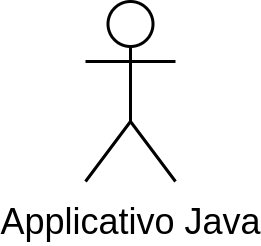
\includegraphics{capitolo3/casi-uso/attori-primari.png}
  \caption{Attori primari}
\end{figure}

\begin{itemize}
  \item \textbf{Applicativo Java}: rappresenta qualsiasi applicazione sviluppata in Java che interagisce con la libreria. In questo caso, consiste nel \textit{back-end} sviluppato utilizzando il \textit{framework} Spring.
\end{itemize}

\subsubsection{Attori secondari}
Un attore secondario è un'entità estranea al sistema che supporta gli attori primari nelle loro attività.

\begin{figure}[h!]
  \centering
  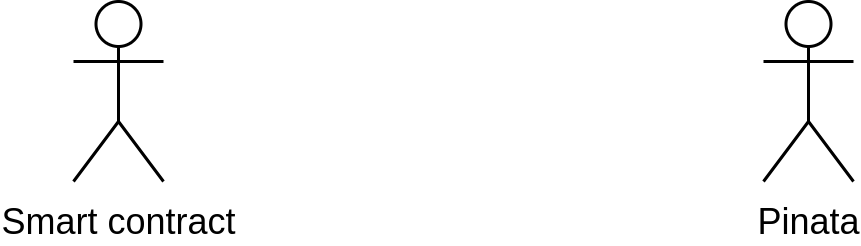
\includegraphics{capitolo3/casi-uso/attori-secondari.png}
  \caption{Attori secondari}
\end{figure}

\begin{itemize}
  \item \textbf{\textit{Smart contract}}: rappresenta lo \textit{smart contract} caricato in \textit{blockchain} con il quale comunicare;
  \item \textbf{Pinata}: rappresenta il servizio che permette di interagire con la rete IPFS.
\end{itemize}

\UC{Caricamento di un opera in blockchain}
Qualsiasi applicativo Java può caricare un opera in blockchain.

\begin{itemize}
  \item \UCPrimaryActors{applicativo Java};
  \item \UCSecondaryActors{\textit{smart contract}, Pinata};
  \item \UCPre{l'applicativo Java vuole creare un NFT da un opera non ancora esistente};
  \item \UCPost{il NFT è stato creato e l'opera è stata caricata nella rete IPFS};
  \item \UCMain
  \begin{itemize}
    \item L'applicativo Java vuole creare un NFT a partire da un opera, dalla quale non è stato creato alcun NFT;
    \item L'opera viene caricata sulla rete IPFS tramite il servizio Pinata;
    \item Viene invocato lo \textit{smart contract} e creato il NFT.
  \end{itemize}
  \item \UCExt
  \begin{enumerate}[label=\lett]
    \item L'applicativo Java vuole assegnare il NFT ad un \textit{wallet} che non è nel formato corretto:
    \begin{itemize}
      \item (UC\ref{UC:extension.wallet-not-correct}) - Visualizzazione messaggio di \textit{wallet} non nel formato corretto;
      \item Viene impedita la creazione del NFT.
    \end{itemize}

    \item L'applicativo Java vuole comunicare con lo \textit{smart contract} attraverso un \textit{wallet}, il quale non è il proprietario di quest'ultimo:
    \begin{itemize}
      \item (UC\ref{UC:extension.operation-not-allowed}) - Visualizzazione messaggio di operazione non consentita;
      \item Viene impedita la creazione del NFT.
    \end{itemize}

    \item L'applicativo Java vuole caricare un'opera dalla quale è già stato estratto il NFT:
    \begin{itemize}
      \item (UC\ref{UC:extension.nft-exists-yet}) - Visualizzazione messaggio di NFT già esistente;
      \item Viene impedita la creazione del NFT.
    \end{itemize}
  \end{enumerate}
\end{itemize}


\UC{Trasferimento della proprietà di un NFT}
L'applicativo Java può trasferire la proprietà di un NFT dal proprietario ad un acquirente.

\begin{itemize}
  \item \UCPrimaryActors{applicativo Java};
  \item \UCSecondaryActors{\textit{smart contract}};
  \item \UCPre{esiste il NFT che si vuole trasferire e l'acquirente è diverso dal proprietario};
  \item \UCPost{il NFT viene trasferito dal proprietario all'acquirente};
  
  \item \UCMain
  \begin{itemize}
    \item L'applicativo Java, attraverso il \textit{wallet} del proprietario dello \textit{smart contract}, comunica con lo \textit{smart contract} caricato nella \textit{blockchain};
    \item Gli invia i dati del proprietario e dell'acquirente;
    \item Viene eseguito il trasferimento.
  \end{itemize}

  \item \UCExt
  \begin{enumerate}[label=\lett]
    \item L'applicativo Java vuole vuole trasferire il NFT dal proprietario all'acquirente, riferendosi ad uno di questi due attraverso un \textit{wallet} che non è nel formato corretto:
    \begin{itemize}
      \item (UC\ref{UC:extension.wallet-not-correct}) - Visualizzazione messaggio di \textit{wallet} non nel formato corretto;
      \item Viene impedito il trasferimento del NFT.
    \end{itemize}

    \item L'applicativo Java vuole comunicare con lo \textit{smart contract} attraverso un \textit{wallet}, il quale non è il proprietario di quest'ultimo:
    \begin{itemize}
      \item (UC\ref{UC:extension.operation-not-allowed}) - Visualizzazione messaggio di operazione non consentita;
      \item Viene impedito il trasferimento del NFT.
    \end{itemize}

    \item L'acquirente corrisponde al proprietario del NFT:
    \begin{itemize}
      \item Visualizzazione messaggio di operazione non andata a buon fine, dato che l'acquirente non può anche essere il proprietario del NFT;
      \item Viene impedito il trasferimento del NFT.
    \end{itemize}
  \end{enumerate}
\end{itemize}

\UC{Ottenimento di un NFT a partire dal suo id}
L'applicativo Java può ottenere le informazioni di un NFT a partire dal id con il quale è memorizzato.

\begin{itemize}
  \item \UCPrimaryActors{applicativo Java};
  \item \UCSecondaryActors{\textit{smart contract}};
  \item \UCPre{l'applicativo Java utilizza un id associato ad un NFT};
  \item \UCPost{l'applicativo Java ottiene le informazioni del NFT};
  \item \UCMain
  \begin{itemize}
    \item l'applicativo Java invoca lo \textit{smart contract} utilizzando un id associato ad un NFT;
    \item riceve le informazioni inserite durante la creazione.
  \end{itemize}

  \item \UCExt
  \begin{enumerate}[label=\lett]
    \item L'applicativo Java invia un id che non è associato ad alcun NFT:
    \begin{itemize}
      \item (UC\ref{UC:extension.nft-not-exists}) - Visualizzazione messaggio di NFT non esistente;
    \end{itemize}
  \end{enumerate}
\end{itemize}

\UC{Ottenimento di un opera a partire dal suo hash}
L'applicativo Java può ottenere le informazioni di un NFT a partire dal hash associato al NFT.

\begin{itemize}
  \item \UCPrimaryActors{applicativo Java};
  \item \UCSecondaryActors{\textit{smart contract}};
  \item \UCPre{l'applicativo Java utilizza un hash associato ad un NFT};
  \item \UCPost{l'applicativo Java ottiene le informazioni del NFT};
  
  \item \UCMain
  \begin{itemize}
    \item l'applicativo Java invoca lo \textit{smart contract} utilizzando il hash associato al NFT;
    \item riceve le informazioni inserite durante la creazione. 
  \end{itemize}
  
  \item \UCExt
  \begin{enumerate}[label=\lett]
    \item l'applicativo Java invia un hash che non è associato ad alcun NFT:
    \begin{itemize}
      \item (UC\ref{UC:extension.nft-not-exists}) - Visualizzazione messaggio di NFT non esistente.
    \end{itemize}
  \end{enumerate}
\end{itemize}

\UC{Ottenimento della storia delle transazioni di un NFT}
L'applicativo Java può ottenere la storia delle transazioni di un NFT a partire dal id con il quale è memorizzato.

\begin{itemize}
  \item \UCPrimaryActors{applicativo Java};
  \item \UCSecondaryActors{\textit{smart contract}};
  \item \UCPre{l'applicativo Java utilizza un id associato ad un NFT};
  \item \UCPost{L'applicativo Java ottiene la storia delle transazioni di un NFT};

  \item \UCMain
  \begin{itemize}
    \item l'applicativo Java invoca lo \textit{smart contract} utilizzando un id associato ad un NFT;
    \item riceve la storia delle transazioni.
  \end{itemize}
  
  \item \UCExt
  \begin{enumerate}[label=\lett]
    \item L'applicativo Java invia un id che non è associato ad alcun NFT:
    \begin{itemize}
      \item (UC\ref{UC:extension.nft-not-exists}) - Visualizzazione messaggio di NFT non esistente;
    \end{itemize}
  \end{enumerate}
\end{itemize}

\UC{Visualizzazione messaggio di wallet non nel formato corretto}
\label{UC:extension.wallet-not-correct}

Nel caso in cui il \textit{wallet} inviato allo \textit{smart contract} non sia nel formato corretto, verrà visualizzato un messaggio di errore che lo segnala.

\begin{itemize}
  \item \UCPrimaryActors{applicativo Java};
  \item \UCSecondaryActors{\textit{smart contract}};
  \item \UCPre{il formato del \textit{wallet} non è nel formato corretto};
  \item \UCPost{viene visualizzato il messaggio che segnala l'errore};
  
  \item \UCMain
  \begin{itemize}
    \item l'applicativo Java invia un \textit{wallet} che non è nel formato corretto;
    \item viene visualizzato il messaggio che segnala l'errore.
  \end{itemize}
\end{itemize}

\UC{Visualizzazione messaggio di operazione non consentita}
\label{UC:extension.operation-not-allowed}

Nel caso in cui lo \textit{smart contract} non venga invocato dal suo proprietario, verrà visualizzato il messaggio di operazione non consentita.

\begin{itemize}
  \item \UCPrimaryActors{applicativo Java};
  \item \UCSecondaryActors{\textit{smart contract}};
  \item \UCPre{lo \textit{smart contract} non viene invocato dal suo proprietario};
  \item \UCPost{viene visualizzato il messaggio di operazione non consentita};
  
  \item \UCMain
  \begin{itemize}
    \item l'applicativo Java non viene invocato dal suo proprietario;
    \item viene visualizzato il messaggio di operazione non consentita. 
  \end{itemize}
\end{itemize}

\UC{Visualizzazione messaggio di NFT già esistente}
\label{UC:extension.nft-exists-yet}

Nel caso in cui si cerchi di caricare un NFT già esistente, verrà visualizzato il messaggio che lo segnalerà.

\begin{itemize}
  \item \UCPrimaryActors{applicativo Java};
  \item \UCSecondaryActors{\textit{smart contract}};
  \item \UCPre{l'applicativo Java carica };
  \item \UCPost{};
  
  \item \UCMain
  \begin{itemize}
    \item 
  \end{itemize}
  
  \item \UCExt
  \begin{enumerate}[label=\lett]
    \item 
  \end{enumerate}
\end{itemize}


\UC{Visualizzazione messaggio di NFT non esistente}
\label{UC:extension.nft-not-exists}

\begin{itemize}
  \item \UCPrimaryActors{applicativo Java};
  \item \UCSecondaryActors{\textit{smart contract}};
  \item \UCPre{}
  \item \UCPost{}
  
  \item \UCMain
  \begin{itemize}
    \item 
  \end{itemize}
  
  \item \UCExt
  \begin{enumerate}[label=\lett]
    \item 
  \end{enumerate}
\end{itemize}

\subsection{Requisiti funzionali}
Tabella dei requisiti funzionali, con relativa spiegazione e fonte.

\subsection{Requisiti di qualità}
Tabella dei requisiti di qualità, con relativa spiegazione e fonte.

\subsection{Requisiti di vincolo}
Tabella dei requisiti di vincolo, con relativa spiegazione e fonte.

%%%%%%%%%%%%%%%%%%%%%%%%%%%%%%%%%%%%%%%%%%%%%%%%%%%%%%%%%%%%%%%%%%%%%%%%%%%%%%%%%

\section{Smart contract per Ethereum}
Spiegazione dello scopo e dei compiti dello smart contract per Ethereum.

\subsection{Progettazione}
Scelte progettuali, best practices impiegate e design pattern che sono stati utilizzati. 

\subsubsection{Architettura}
Presentazione dell'architettura con diagrammi di package, classe e sequenza.

\subsection{Codifica}
Spiegazione di quanto fatto durante il periodo di codifica, approfondendo parti di codice che ritengo importanti.

\subsection{Verifica}
Spiegazione delle librerie attraverso le quali sono stati implementati i test, numero di test scritti e code coverage raggiunto.

%%%%%%%%%%%%%%%%%%%%%%%%%%%%%%%%%%%%%%%%%%%%%%%%%%%%%%%%%%%%%%%%%%%%%%%%%%%%%%%%%

\section{Lo standard ERC721 per Hotmoka}
Spiegazione del perché è risultata necessaria la scrittura dello standard ERC721 per Hotmoka.

\subsection{Progettazione}
Scelte progettuali, best practices impiegate e design pattern che sono stati utilizzati. 

\subsubsection{Architettura}
Presentazione dell'architettura con diagrammi di package, classe e sequenza.

\subsection{Codifica}
Spiegazione di quanto fatto durante il periodo di codifica, approfondendo parti di codice che ritengo importanti.

\subsection{Verifica}
Spiegazione delle librerie attraverso le quali sono stati implementati i test, numero di test scritti e code coverage raggiunto.

%%%%%%%%%%%%%%%%%%%%%%%%%%%%%%%%%%%%%%%%%%%%%%%%%%%%%%%%%%%%%%%%%%%%%%%%%%%%%%%%%

\section{Smart contract per Hotmoka}
Spiegazione dello scopo e dei compiti dello smart contract per Hotmoka.

\subsection{Progettazione}
Scelte progettuali, best practices impiegate e design pattern che sono stati utilizzati. 

\subsubsection{Architettura}
Presentazione dell'architettura con diagrammi di package, classe e sequenza.

\subsection{Codifica}
Spiegazione di quanto fatto durante il periodo di codifica, approfondendo parti di codice che ritengo importanti.

\subsection{Verifica}
Spiegazione delle librerie attraverso le quali sono stati implementati i test, numero di test scritti e code coverage raggiunto.

%%%%%%%%%%%%%%%%%%%%%%%%%%%%%%%%%%%%%%%%%%%%%%%%%%%%%%%%%%%%%%%%%%%%%%%%%%%%%%%%%

\section{Libreria per l'integrazione con gli smart contract}
Spiegazione dello scopo e dei compiti della libreria per l'integrazione con gli smart contract.

\subsection{Progettazione}
Scelte progettuali, best practices impiegate e design pattern che sono stati utilizzati. 

\subsubsection{Architettura}
Presentazione dell'architettura con diagrammi di package, classe e sequenza.

\subsection{Codifica}
Spiegazione di quanto fatto durante il periodo di codifica, approfondendo parti di codice che ritengo importanti.

\subsection{Verifica}
Spiegazione delle librerie attraverso le quali sono stati implementati i test, numero di test scritti e code coverage raggiunto.

%%%%%%%%%%%%%%%%%%%%%%%%%%%%%%%%%%%%%%%%%%%%%%%%%%%%%%%%%%%%%%%%%%%%%%%%%%%%%%%%%

\section{Validazione e collaudo}
Riassunto dei requisiti soddisfatti e risultato del collaudo.

%%%%%%%%%%%%%%%%%%%%%%%%%%%%%%%%%%%%%%%%%%%%%%%%%%%%%%%%%%%%%%%%%%%%%%%%%%%%%%%%%

\section{Resoconto dei prodotti sviluppati}
Quantità di prodotti software che sono stati sviluppati (in termini di linee di codice) e numero di documenti prodotti.

%%%%%%%%%%%%%%%%%%%%%%%%%%%%%%%%%%%%%%%%%%%%%%%%%%%%%%%%%%%%%%%%%%%%%%%%%%%%%%%%%

\section{Integrazione del prodotto in NFTLab}
Come quanto è stato implementato si integra all'interno del prodotto NFTLab.

%%%%%%%%%%%%%%%%%%%%%%%%%%%%%%%%%%%%%%%%%%%%%%%%%%%%%%%%%%%%%%%%%%%%%%%%%%%%%%%%%

\section{Le conclusioni}
Considerazioni conclusive sul confronto tra le due blockchain Hotmoka e Ethereum.
